\documentclass[12pt]{article}

\usepackage{../thesis}

\usepackage[americaninductors]{circuitikz}
\usetikzlibrary{decorations.pathmorphing}

\begin{document}

\pagestyle{empty}

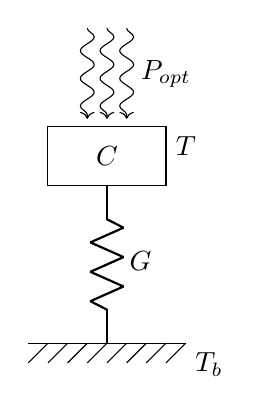
\begin{tikzpicture}
    % First the light falling on the bolometer
	\draw [->] decorate [decoration={snake}] {(-0.25,4.0) -> (-0.25,2.85)};
	\draw [->] decorate [decoration={snake}] {( 0.00,4.0) -> ( 0.00,2.85)};
	\draw [->] decorate [decoration={snake}] {( 0.25,4.0) -> ( 0.25,2.85)};
	\draw (0.75, 3.425) node {$P_{opt}$};
    
    % Now the thermal link and heat capacity
    \draw (0,2) to[R, l=$G$] (0,0);
    \draw (-0.75,2) rectangle (0.75,2.75) node[midway] {$C$} node[below right] {$T$};
    
    % Now the temperature bath
    \draw (-1,0) -- (1,0) node[below right] {$T_b$};
    \draw (-1.00,-0.25) -- (-0.75,0);
    \draw (-0.75,-0.25) -- (-0.50,0);
    \draw (-0.50,-0.25) -- (-0.25,0);
    \draw (-0.25,-0.25) -- (-0.00,0);
    \draw ( 0.00,-0.25) -- ( 0.25,0);
    \draw ( 0.25,-0.25) -- ( 0.50,0);
    \draw ( 0.50,-0.25) -- ( 0.75,0);
    \draw ( 0.75,-0.25) -- ( 1.00,0);
    
\end{tikzpicture}

\end{document}
